\documentclass[titlepage]{article}
\usepackage{graphicx} % Required for inserting images

\title{Recursividad-Iteratividad en Mips32}
\author{Cesar Rojas, \#31406902}
\date{Julio 2025}

\begin{document}

\maketitle

\section*{¿Como se implementa la recursividad en Mips32? ¿Que papel cumple la pila (\$sp)?}

Un procedimiento recursivo es un tipo de procedimiento anidado que se invoca a si mismo repetidamente hasta satisfacer una condición. En Mips32 los procedimientos recursivos se llaman asi mismos usando los registros de argumento (\emph{\$a1-\$a3}), pero debido a que la llamada ocurre antes de que el procedimiento recursivo original termine, ocurre un conflicto con el uso de los registros de argumento ademas de con el \emph{Return Adress} (\emph{\$ra}).

Para implementar procedimientos recursivos en Mips32 es necesario guardar tanto el \emph{Return Adress} como los registros de argumento en la pila. De esta forma una vez la llamada recursiva termine de ejecutarse, estos se pueden volver a cargar a su valor original guardado en la pila para que el procedimiento recursivo pueda continuar normalmente.

La pila también se usa para guardar las variables del procedimiento que no caben en los registros.

\section*{¿Que riesgos de desbordamiento existen? ¿Como mitigarlos?}

El principal riesgo de desbordamiento es la pila. Es necesario asegurarse de manipular el tamaño de esta correctamente, guardar y cargar en las posiciones correctas, y de restaurar los registros correctamente después de una llamada recursiva.

\section*{Diferencia entre una implementación iterativa y recursiva en cuanto al uso de memoria y registros}

Un procedimiento iterativo es usualmente mas eficiente que una procedimiento recursivo, ofreciendo mayores prestaciones ya que se elimina el costo de llamar al procedimiento una y otra vez. 

Las implementaciones recursivas usan mucho mayormente a la pila de memoria, ya que esta se incrementa por cada llamada recursiva subsecuente para guardar las direcciones de retorno y registros para no perder las variables del procedimiento.

En contraste, una implementación iterativa suele depender mucho menos en la pila mas alla de guardar los registros a utilizar y aquellas variables adicionales que no quepan en los registros.

\section*{Diferencia entre los ejemplos del libro y un ejercicio completo en Mips32}

La mayor diferencia cae en la \emph{preparación} y el \emph{resultado}. Los ejercicios del libro no tocan en lo que es necesario antes de llamar a un procedimiento recursivo, ni muestras los segmentos del programa (\emph{.data} y \emph{.text}).

Antes de llamar a un procedimiento recursivo es necesario asignar valores a los registros de argumento, y una vez este se termine de ejecutar es importante guardar el retorno (\emph{\$v0}) en otro registro inmediatamente para evitar sobre-escribirlo.

\section*{Realización de la ejecución paso a paso en MARS de la implementación iterativa}

Primero, preparamos un arreglo donde guardaremos nuestra secuencia. reservamos 46 espacios ya que a partir de la posición 47, los números de la secuencia de Fibonacci son demasiado grandes para los registros.\\

\noindent .data\\
	array: .space 184 \# 184 = 46 * 4 (Fibonacci 47 es demasiado grande para los registros)\\

Luego, leemos un numero como entrada del usuario. Este sera la posición de la secuencia de Fibonacci a la que queremos llegar.\\

\noindent .text\\
	\# Leer entrada del usuario\\
	li \$v0, 5 \# Leer entero\\
	syscall\\

Guardamos este valor, y la dirección de nuestro arreglo, como argumentos para nuestro procedimiento Fibonacci, y luego lo llamamos.\\

\noindent \# Toma como argumentos la posición a la que llegar y la dirección del arreglo\\
	addi \$a0, \$v0, 0\\
	la \$a1, array\\
	jal fibonacci\\

Una vez dentro de nuestro procedimiento, guardaremos el numero 1 dentro del arreglo \$t0. Este servira como la 'i' (el indice) de nuestro bucle.\\

\noindent fibonacci:\\
	li \$t0, 1 \# Contador\\

Ya que los primeros dos números de la secuencia son ambos 1, guardamos este numero de forma inmediata en las primeras dos posiciones de nuestro arreglo.\\
	
\noindent \# Guardar el numero 1 en la primera y segunda posición (los primeros dos números de la secuencia son 1)\\
	sw \$t0, 0(\$a1)\\
	sw \$t0, 4(\$a1)\\
	addi \$a1, \$a1, 4 \# Mover el apuntador un espacio hacia arriba\\
	addi \$t0, \$t0, 1 \# Aumentar el contador en uno\\

Después, empieza nuestro bucle, donde iteramos por las posiciones de la secuencia de Fibonacci hasta llegar al numero 'n' que nos proveyó el usuario como entrada. ( for(int i = 2; i < n; i++ ) ) donde 'i' es \$t0 y 'n' es \$a0.\\

\noindent \# Empezamos el bucle\\
	loop:\\
		bge \$t0, \$a0, exitLoop \# Si \$t0 >= \$a0, salir del bucle\\

Dentro del bucle, cargamos la posición actual y la posición anterior en dos registros. Luego, los sumamos juntos y los guardamos en la posición siguiente.\\
        
\noindent lw \$t1, 0(\$a1)\\
		lw \$t2, -4(\$a1)\\
		add \$t1, \$t1, \$t2 \# Sumar los dos últimos números de la secuencia\\
		sw \$t1, 4(\$a1) \# Guardar el resultado como el siguiente numero de la secuencia\\

Una vez realicemos esto, incrementamos la posición actual en uno, e igual con nuestro indice de bucle 'i' antes de volver a repetir el bucle.\\
		
\noindent addi \$a1, \$a1, 4 \# Mover el apuntador un espacio hacia arriba\\
		addi \$t0, \$t0, 1 \# Aumentar el contador del bucle\\
		j loop \# Repetir el bucle\\

Finalmente, una vez salgamos del bucle, guardamos la dirección de la ultima posicion en \$v0 para retornarla como el resultado del procedimiento.\\

\noindent exitLoop:\\
		addi \$v0, \$a1, 0 \# Retornar la ultima posición en \$v0\\
		jr \$ra\\

Luego, volvemos a la posición donde se llamo el procedimiento. Simplemente guardamos el retorno en \$s0 y lo imprimimos por pantalla.\\

\noindent \# Retorna la ultima posición en \$v0\\
	addi \$s0, \$v0, 0\\
    \# Escribir el resultado por pantalla\\
	li \$v0, 1\\
	lw \$a0, 0(\$s0)\\
	syscall\\
	\# Salir del programa\\
	li \$v0, 10\\
	syscall\\

\section*{Selección de enfoque}

Elegir realizar un procedimiento de manera recursiva o iterativa depende de varios factores, como la eficiencia, la claridad de código, la complejidad y el proposito del procedimiento.

Usualmente, los procedimientos iterativos son mas eficientes en cuanto a prestaciones y son mas fáciles de leer y entender, gracias a su uso de etiquetas con nombres (idealmente) descriptivos.

Sin embargo, no siempre es mas eficiente (o incluso, \emph{posible}) realizar un procedimiento iterativamente. Existen casos donde una implementación recursiva posee una complejidad menor a la de una implementación iterativa equivalente.

Por lo tanto, es importante analizar con cuidado el propósito de nuestro procedimiento para si elegir efectivamente el tipo de implementación.

\section*{Análisis y discusión de resultados}

Al ejecutarse, tanto la implementación iterativa como recursiva retornan el mismo resultado, este siendo el numero ubicado en la posición de la secuencia que le demos al programa como entrada.

Al ingresar 1 o 2, el programa retornara el numero 1. Esto es debido a que los primeros dos números de la secuencia de Fibonacci son ambos el numero 1.

Nuestros procedimientos por lo tanto guarda este numero en las primeras dos posiciones al llamarse inicialmente.

Si se ingresa un numero menor a 1 como entrada (posiciones negativas) el programa retornara el numero 1 de forma igual.

Cualquier entrada mayor a 2 retornara la suma de los números en las ultimas dos posiciones. Por lo tanto, al ingresar 3 como entrada, el programa nos devolverá 2, e ingresar 8, devolverá 21.

\begin{figure}[h]
    \centering
    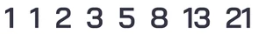
\includegraphics[width=0.75\textwidth]{images/fibonacci.png} % 75% of text width
    \label{fig:step1}
\end{figure}

Ingresar un numero mayor a 46 causara un error de desbordamiento, ya que intentaría retornar un numero demasiado grande para nuestro registro de retorno.

\end{document}
